\subsection{Extra dimensie}
Laten we een één-dimensionaal kanaal beschouwen waarin we een concentratie noteren met $c(\vec{x},t)$. We nemen aan dat het kanaal zo dun is in de $y$ en $z$ richting dat we kunnen stellen dat $c(\vec{x},t)=c(x,t)$. Zie figuur \ref{fig:xchannel}

\begin{figure}[h]
	\centering
	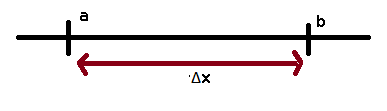
\includegraphics[]{DeltaX.png}
	\label{fig:xchannel}
	\caption{Stukje van het één dimensionale kanaal}
\end{figure}

Beschouw nu een interval $I_x$ tussen $x$ en $x+\Delta x$ met $\Delta x > 0$, dus $I_x = [x, x+\Delta x]$. De totale hoeveelheid stof verandert doordat er ofwel een netto flux is over de randen, ofwel er is bron. Naast dat er interne veranderingen zijn zoals beschreven in het model van Evans \& Parslow \cite{Algen1985}, introduceert de extra dimensie twee nieuwe factoren die verandering van concentratie teweeg brengt, namelijk stroming en diffusie. In de volgende twee paragrafen wordt afgeleid hoe deze factoren de concentratie distributie be\"{i}nvloeden.

\subsubsection{Diffusie}
De totale hoeveelheid stof $M(x,t)$ in het interval $I$ wordt gegeven door de volgende vergelijking
\begin{equation}
	M(x,t) = \int_x^{x+\Delta x} c(\tilde{x})\dif \tilde{x} \approx c(x)\Delta x
\end{equation}
hier is aangenomen dat $\Delta x$ erg klein is en $c$ voldoende glad zodat $c(\tilde{x}) \approx c(x)$ voor $\tilde{x} \in I_x$. Vervolgens kijken we naar de diffusie. Ficks wet stelt dat de diffusie flux $J$ proportioneel is met de negatieve gradient van de concentratie met proportionaliteitsconstante $D$. Dit betekent
\begin{equation}
	\vec{J}(\vec{x},t) = -D\cdot  \nabla c(\vec{x},t) \overEquals{1D} -D\cdot \dd{x} c(x,t).
\end{equation}
De concentratie binnen het kanaal verandert dus doordat er een influx is aan de randen, deze is gegeven door
\begin{equation}
	\phi_{\text{D}}(t) = \oint_{\partial I} \vec{J}(\vec{x},t)\cdot \dif \vec{S} \oneD J(a,t)-J(b,t) = -D\bigg(\dd{c}{x}(a,t) - \dd{c}{x}(b,t)\bigg)
\end{equation}

Hieruit volgt dat 
\begin{equation}
     \frac{d}{dt}{M}(t) = \dd{}{t} \bigg(c(x) A \Delta x\bigg) = A\phi_{D}(t) = -AD\bigg(\dd{C}{x}(a,t) - \dd{c}{x}(b,t)\bigg)
\end{equation}
\begin{equation}
    \dd{C}{t} \approx  \frac{D\bigg(\dd{c}{x}(x+\Delta x,t) - \dd{C}{x}(x,t)\bigg)}{\Delta x}
\end{equation}
en als we nu de limiet van $\Delta x$ naar nul nemen vinden we 
\begin{equation}
    \dd{c}{t}(x,t) = \dd{}{x}D\dd{c}{x} \overEquals{*} D\ddn{c}{x}{2}
\end{equation}
waar we bij (*) hebben aangenomen dat het medium zeewater zo goed als homogeen is en $D$ als constante beschouwd kan worden.

\newpage
\subsubsection{Stroming}
Voor stroming kunnen we een zelfde soort aanpak gebruiken als bij diffusie. Echter, nu is de vergelijking voor de flux anders. We hebben
\begin{equation}\phi_{in} = \vec{\phi}''_{in}  \cdot \vec{A}(x)=  c(x)\vec{V}(x) \cdot \vec{A}(x)
\label{eq:currentFlux1}
\end{equation}
\begin{equation}\phi_{out} = \vec{\phi}''_{out}\cdot \vec{A}(x+\Delta x) = c(x+\Delta x)\vec{V}(x+\Delta x) \cdot \vec{A}(x+\Delta x)
\label{eq:currentFlux2}
\end{equation}
Waar de accenten de ruimtelijke dimensie aangeeft, dus één accent betekent per lengte-eenheid, twee accenten per oppervlakte-eenheid, enzovoorts. Omdat $\vec{V} \perp \vec{A} \quad \forall \tilde{x} \in [0,L]$ kunnen we vergelijkingen \ref{eq:currentFlux1} en \ref{eq:currentFlux2} reduceren naar simpele producten. De tijdsafgeleide van de totale hoeveelheid stof is dus
\begin{equation}
    \dd{M}{t}(x,t) \approx A\Delta x\frac{\partial c}{\partial t} =  \phi_{in} - \phi_{out} = c(x)V(x)A - c(x+\Delta x)V(x+\Delta x)A
\end{equation} 
\begin{equation} \frac{\partial c}{\partial t} =  \frac{c(x)V(x) - c(x+\Delta x)V(x+\Delta x)}{\Delta x}
\end{equation}
\begin{equation} \frac{\partial c}{\partial t} =  \frac{\partial c}{\partial x}(x)V(x) + c(x)\cancelto{0}{\frac{\partial V}{\partial x}(x)} = \frac{\partial c}{\partial x}(x)V(x)
\end{equation}

\textbf{TO BE CONTINUED - JB, ik wil dit bovenste ook nog verbeteren. Heb het gevoel dat het rigoreuzer kan door met willekeurige $a,b$ te werken}